\documentclass[11pt,a4paper,bibliography=totocnumbered]{scrartcl}
\usepackage[utf8]{inputenc}
\usepackage[british]{babel}
%\usepackage{amsmath}
%\usepackage{amsfonts}
%\usepackage{amssymb}
\usepackage[footsepline]{scrlayer-scrpage}
\usepackage{tabu}
\usepackage{placeins}
%\usepackage{longtable}
\usepackage{multirow}
\usepackage{setspace}
%\usepackage{graphicx}
%\usepackage{pgfplots}
\usepackage{hyperref}
\usepackage{url}
\usepackage{titling}
\usepackage[backend=biber,sorting=none]{biblatex}
\usepackage{csquotes}
\usepackage{pdfpages}
\usepackage{epstopdf}
\usepackage{graphicx}
\usepackage{subfig}
\usepackage{array}
%\usepackage{enumitem}
\usepackage[backgroundcolor=lightgray]{todonotes}

%\pgfplotsset{width=12cm,height=6cm,compat=1.11}

% Constants
\def\mytitle{Tomcat Native 2}
\def\myauthor{Jocelyn Thode and Simon Brulhart}
\def\theclient{Red Hat}

\pagestyle{scrheadings}

\ihead{\mytitle}
\chead{}
\cfoot{}
\ifoot{Initial plan}
\ofoot{\thepage}

\posttitle{\end{center}\begin{center}\LARGE Final Report\end{center}}

\author{\myauthor\\ \href{mailto:jocelyn.thode@unifr.ch}{jocelyn.thode@unifr.ch} \\ \href{mailto:simon.brulhart@unifr.ch}{simon.brulhart@unifr.ch}}
\title{\huge \textbf{\mytitle}}

\bibliography{final_report}

\begin{document}

\graphicspath{{figures/}}

\begin{titlingpage}

\maketitle

\begin{abstract}
\mytitle{} is a project mandated by Red Hat. It aims at providing a JNI wrapper for OpenSSL for use in both Undertow and Tomcat. This project is the practical part of the R\&D Workshop course given at the University of Neuchâtel as part of the Joint Master in Computer Science.
\end{abstract}

\begin{figure}[b]
\centering
\subfloat{
\includegraphics[height=1.8cm]{unine.eps}}
\qquad
\subfloat{
\includegraphics[height=1.5cm]{jmcs.png}}
\qquad
\subfloat{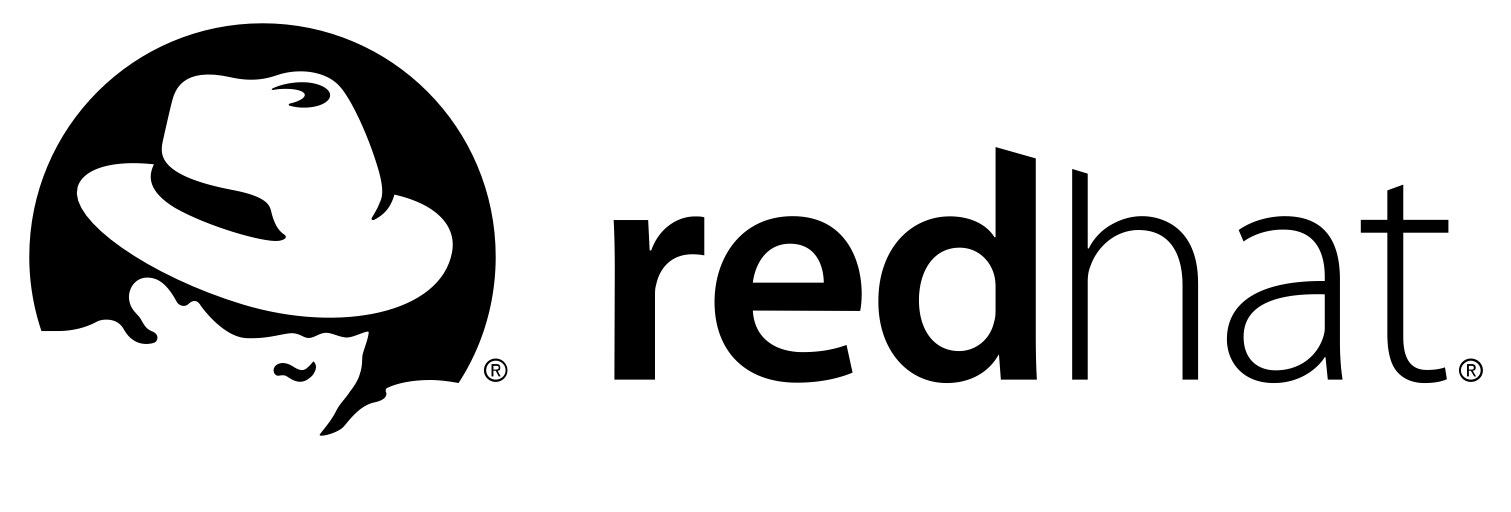
\includegraphics[height=1.6cm]{redhat-logo.png}}
\end{figure}

\end{titlingpage}

\pagebreak

\setcounter{tocdepth}{2}
\tableofcontents
\listoffigures

\pagebreak

\section{Project description}

\subsection{Project context}
For this project we are working with \theclient{} which is a multinational software company that provides open-source software and technical support to enterprises\autocite{redhat}.
At the moment, Tomcat\autocite{tomcat} and Undertow\autocite{undertow} are among the most used Java web servers. Both rely on TLS/SSL to encrypt and secure communications between a client and a server. To achieve good performance Tomcat Native\autocite{tomcat-native} provides access to OpenSSL in Tomcat. It uses Apache Portable Runtime (APR) to do so. 
Unfortunately, Undertow isn't compatible with Tomcat Native at the moment.
Until last year, the APR would manage the encrypted sockets by itself. However this implied a lot of C code to maintain. To ease maintenance, some work has been done to use OpenSSL APIs directly instead. This works well enough despite some acceptable performance penalty. However the APR still provides the bindings to these APIs.
We now want to strip the current solution of the APR and make the result compatible with Undertow.

Figure \ref{fig:current} shows an overview of the different ways to use TLS/SSL in Tomcat. This figure describes the path taken by a piece of data, going from Tomcat/Undertow to the OS network layer. There is a different color for each way to use TLS/SSL. We describe the architecture in more detail in Section \ref{sec:architecture}.

\subsection{Goals and objectives of the project}

Our project aims to refactor Tomcat Native to drop APR and only rely on our own JNI\footnote{Java Native Interface} wrapper to interface with OpenSSL. This should make Tomcat Native much more maintainable while keeping great performance when using TLS/SSL. The project also aims to make the resulting \mytitle{} usable in Undertow while keeping the compatibility with Tomcat.
This means we need to :
\begin{enumerate}
\item Study the source code of Tomcat Native, Undertow and some experiments already done to use OpenSSL in Undertow.
\item Remove all APR code present in Tomcat Native
\item Abstract Tomcat Native to be used in Tomcat and Undertow
\item Provide good documentation so that the open-source community can use the project
\item Run benchmarks to test the implementation on multiple platforms
\item Merge OpenSSL 1.1 in \mytitle{}
\item Extend the OpenSSL support by adding JNIs for more features
\end{enumerate}

Figure \ref{fig:goal} shows what is expected at the end of the project.

\section{Project organization}
\label{sec:org}

This project requires us to read some documentation and source code. We also need to write reports and presentations. To keep the code base clean, we decided to adopt the same strategy as Numa de Montmollin last year and split our work in two different repositories on Github.

\href{https://github.com/jocelynthode/tomcat-native2-doc}{tomcat-native2-doc} is the repository documenting the progress of our project. We put every report and presentation in the repo. This repo also contains a wiki which hosts the logbook, work plan and our different articles. The articles are useful to share our findings and more importantly to not forget about them.

\href{https://github.com/jocelynthode/tomcat-native2}{tomcat-native2} is the repository dedicated to the code. This repo includes our implementation, and the documentation directly concerning it. For example, it should contain a ReadMe describing the building process and the main purpose of the project.

\section{Realization}
The project was realized as follows: \mytitle{} is built as a common code base between Undertow and Tomcat. It should be optionally compiled on the side and loaded at run-time if the user needs to use the OpenSSL engine.

For this purpose, we needed to move some Tomcat code related to Tomcat-Native into our repo. Unfortunately the entire Java code could not be the same in Undertow and Tomcat. The reasons are explained in the section \ref{sec:issues}.

The C code used in \mytitle{} does not rely on APR anymore. It only works under POSIX compatible systems for now. \mytitle{} is working with OpenSSL up to 1.1. To use \mytitle{} one needs to build the native and java parts and then include the generated jar as a dependency on both Tomcat and Undertow.

In Undertow, a sample example has been provided to showcase how to use \mytitle{} together with the web server.

In Tomcat, simply using the NIO.2 or NIO connector should work when explicitly using \mytitle{}.

\subsection{Build}
\subsubsection{\mytitle{}}
\begin{enumerate}
	\item \begin{verbatim}ant jar\end{verbatim}
	\item \begin{verbatim}cd native\end{verbatim}
	\item \begin{verbatim}./buildconf && ./configure && make\end{verbatim} (\texttt{make} might return an error because it tries to install the libraries after building them, but this is not important)
\end{enumerate}
\subsubsection{Tomcat}
\begin{enumerate}
	\item \begin{verbatim}TCN2=path/to/tomcat-native-repository\end{verbatim}
	\item \begin{verbatim}git clone https://github.com/jocelynthode/tomcat.git && cd tomcat\end{verbatim}
	\item \begin{verbatim}git checkout undercat_trunk\end{verbatim}
	\item \begin{verbatim}echo "tcn2.jar=$TCN2/dist/tomcat-native-1.2.8.jar" >> build.properties\end{verbatim}
	\item \begin{verbatim}ant\end{verbatim}
\end{enumerate}
\subsubsection{Undertow}
\begin{enumerate}
	\item \begin{verbatim}TCN2=path/to/tomcat-native-repository\end{verbatim}
	\item \begin{verbatim}git clone https://github.com/jocelynthode/undertow.git && cd undertow\end{verbatim}
	\item \begin{verbatim}git checkout undercat_trunk\end{verbatim}
	\item \begin{verbatim}./deps.sh "$TCN2"\end{verbatim}
	\item \begin{verbatim}mvn package -DskipTests -Dcheckstyle.skip\end{verbatim}
\end{enumerate}
The build process is also available in more details on the ReadMe of the \mytitle{} repository, as well as specific instructions to run the obtained builds.

\section{Architecture}
\label{sec:architecture}
\subsection{State Of The Art}
Currently there are 3 ways to use SSL/TLS in Tomcat, as shown on Figure \ref{fig:current}. The first one uses the OpenSSL through the APR connector (blue path). Here the APR handles encryption and networking. It provides its own socket API and transparently encrypts and decrypts data flowing through it. Since the APR is programmed in C, Tomcat-Native offers JNIs to be used in Tomcat.

The second way (brown and black path) uses an NIO/NIO.2 connector with the JSSE engine, included in Java standard library. This has the benefit of using no external dependency. However the JSSE engine is not native code, which makes it the slowest option for SSL/TLS. Note that JSSE also provides a networking API, but Tomcat uses NIO/NIO.2 instead.

The third way (red and black path) also uses an NIO/NIO.2 connector, but it uses OpenSSL instead of JSSE for encryption. For this OpenSSL engine, Tomcat provides Java classes implementing the JSSE API. Then these classes call OpenSSL functions through the JNIs offered in Tomcat Native. However, the JNIs still use some features of the APR behind the scene, such as portable memory management. As explained in previous sections, this way was implemented last year with the goal of replacing the APR connector.

Concerning encryption, Undertow follows a similar architecture as the second way (NIO/NIO2 with JSSE engine).

\subsection{Tomcat Native 2}
Figure \ref{fig:goal} describes the architecture of \mytitle{} after our changes. We got rid of the APR connector and don't use the APR in JNIs anymore. Most of the Java code concerning the OpenSSL engine was moved from Tomcat to \mytitle{} so that Undertow can use it. However Tomcat and Undertow use a different system to provide and instantiate the OpenSSL engine. These differences are explained in section \ref{sec:issues}. To fix this issue, we kept slightly different versions of some classes in both projects.

\section{Results}
\todo[inline] {here speak about benchmarks}
\begin{figure}[!h]
	\begin{center}
		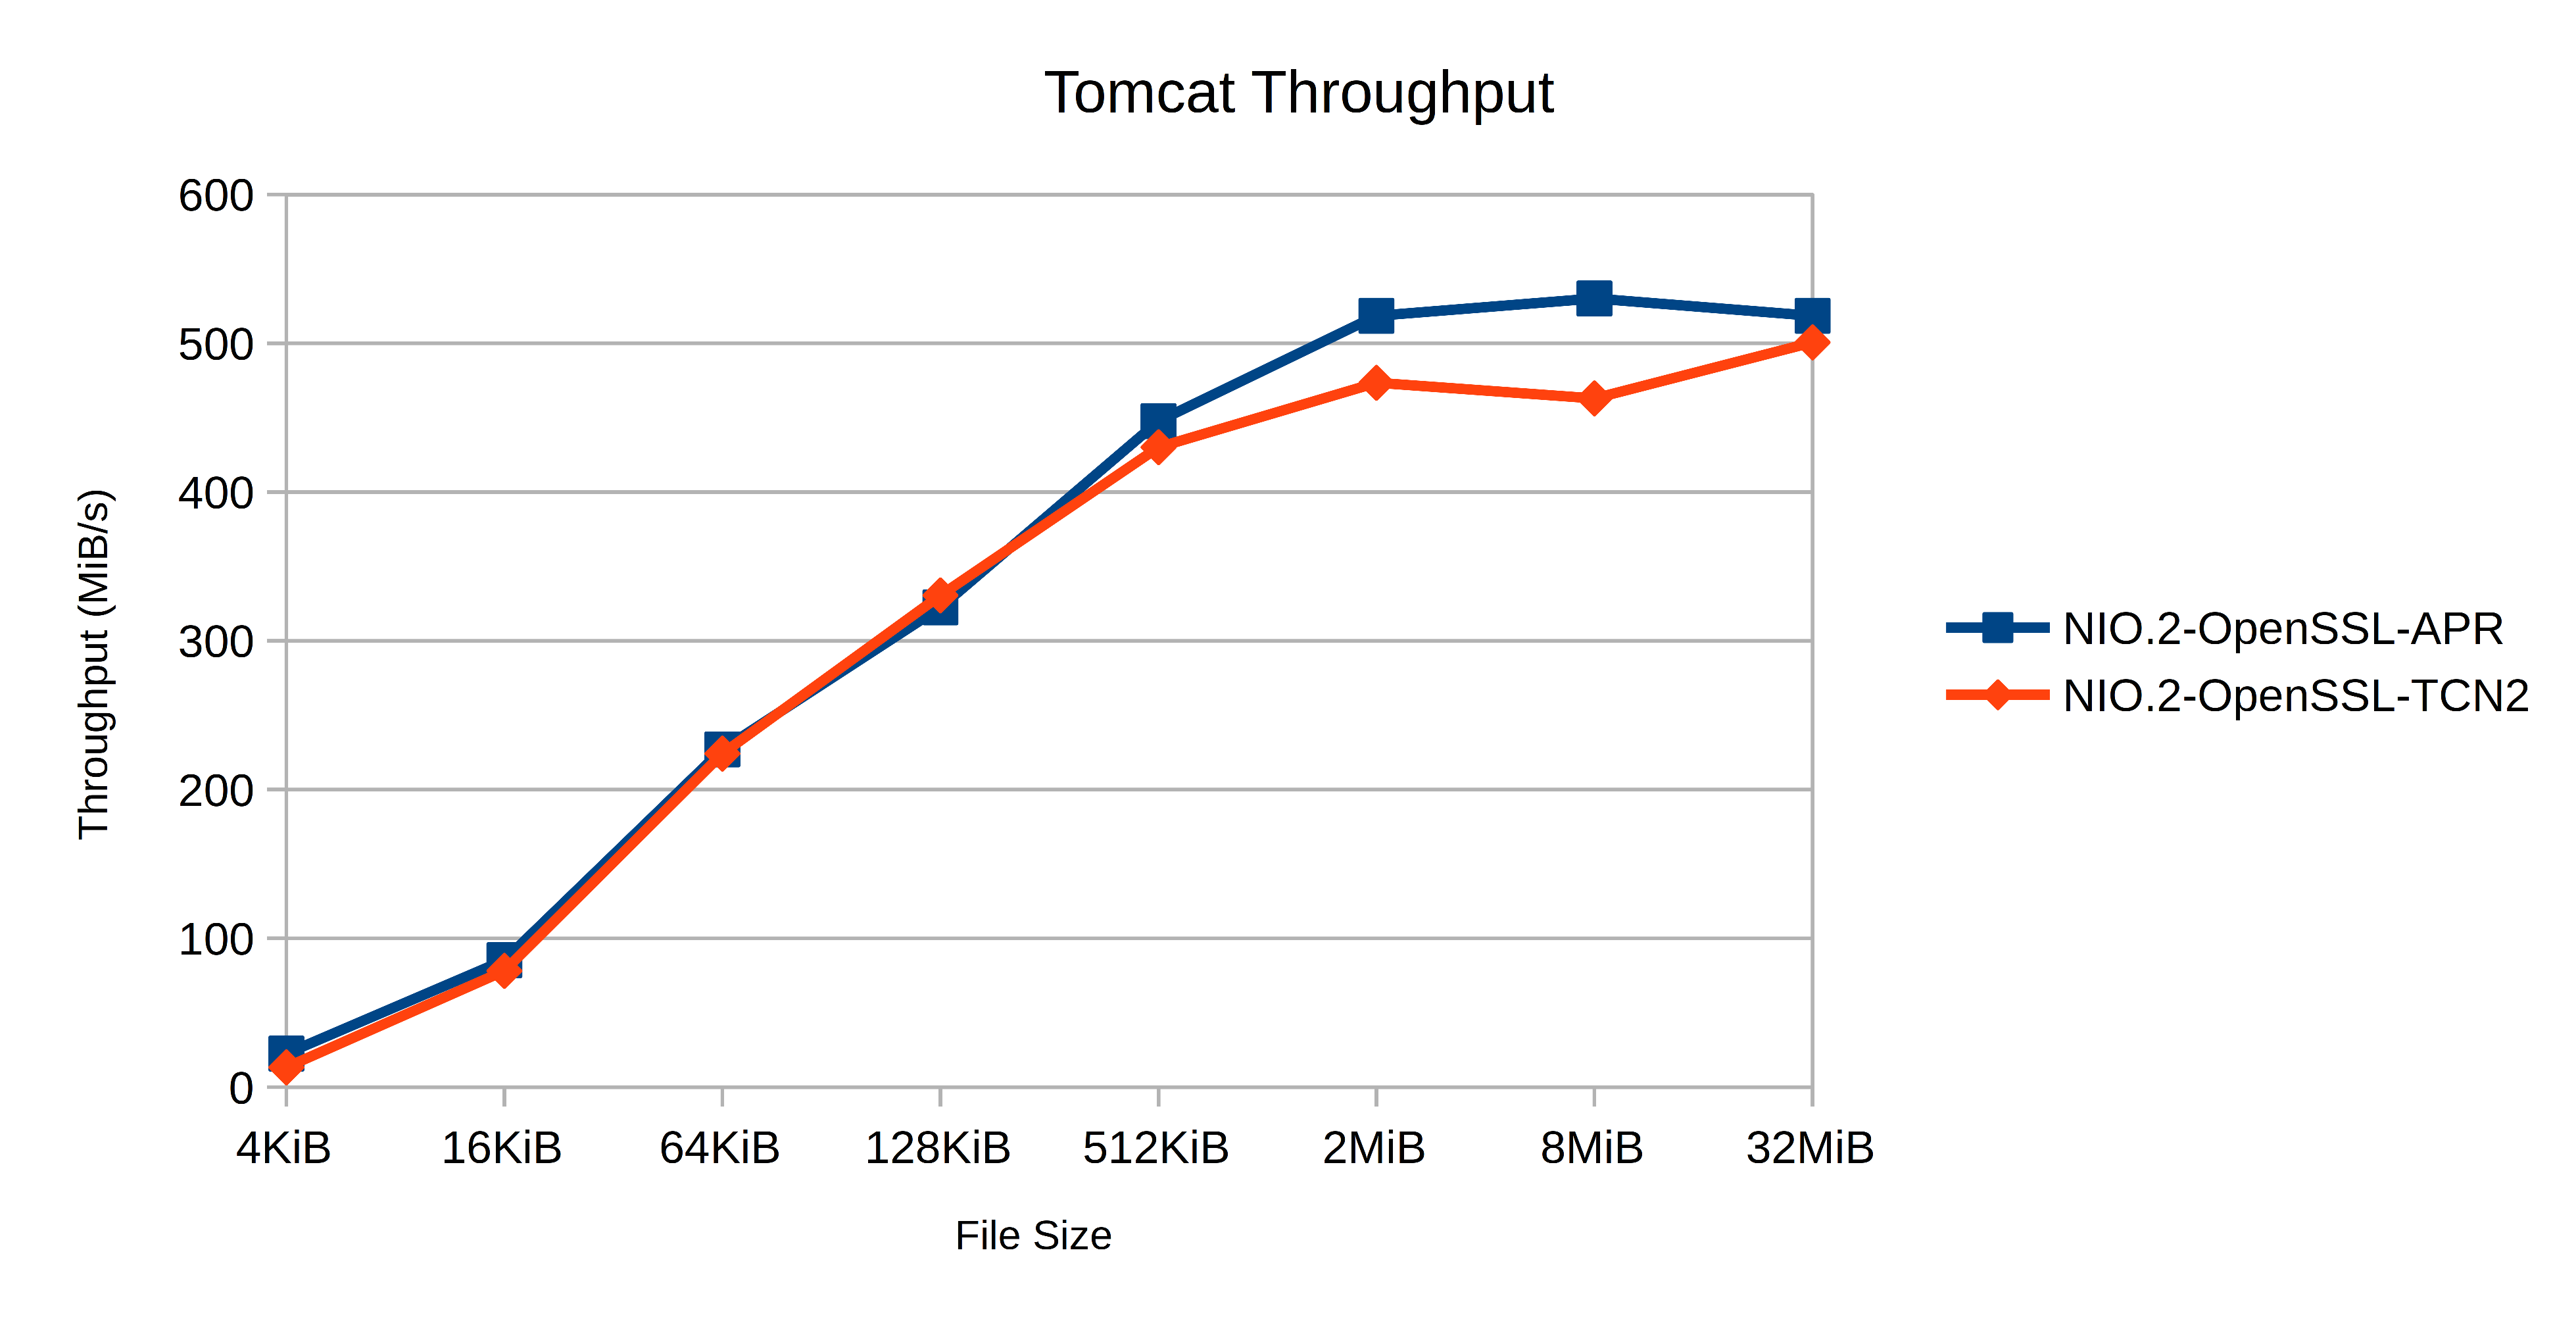
\includegraphics[scale=0.23]{tomcat-throughput.pdf}
	\end{center}
	\caption{\textbf{Diagram showing the difference in throughput between Tomcat with \mytitle{} and Tomcat with Tomcat Native. }}
	\label{fig:tomcat-throughput}
\end{figure}

\begin{figure}[!h]
	\begin{center}
		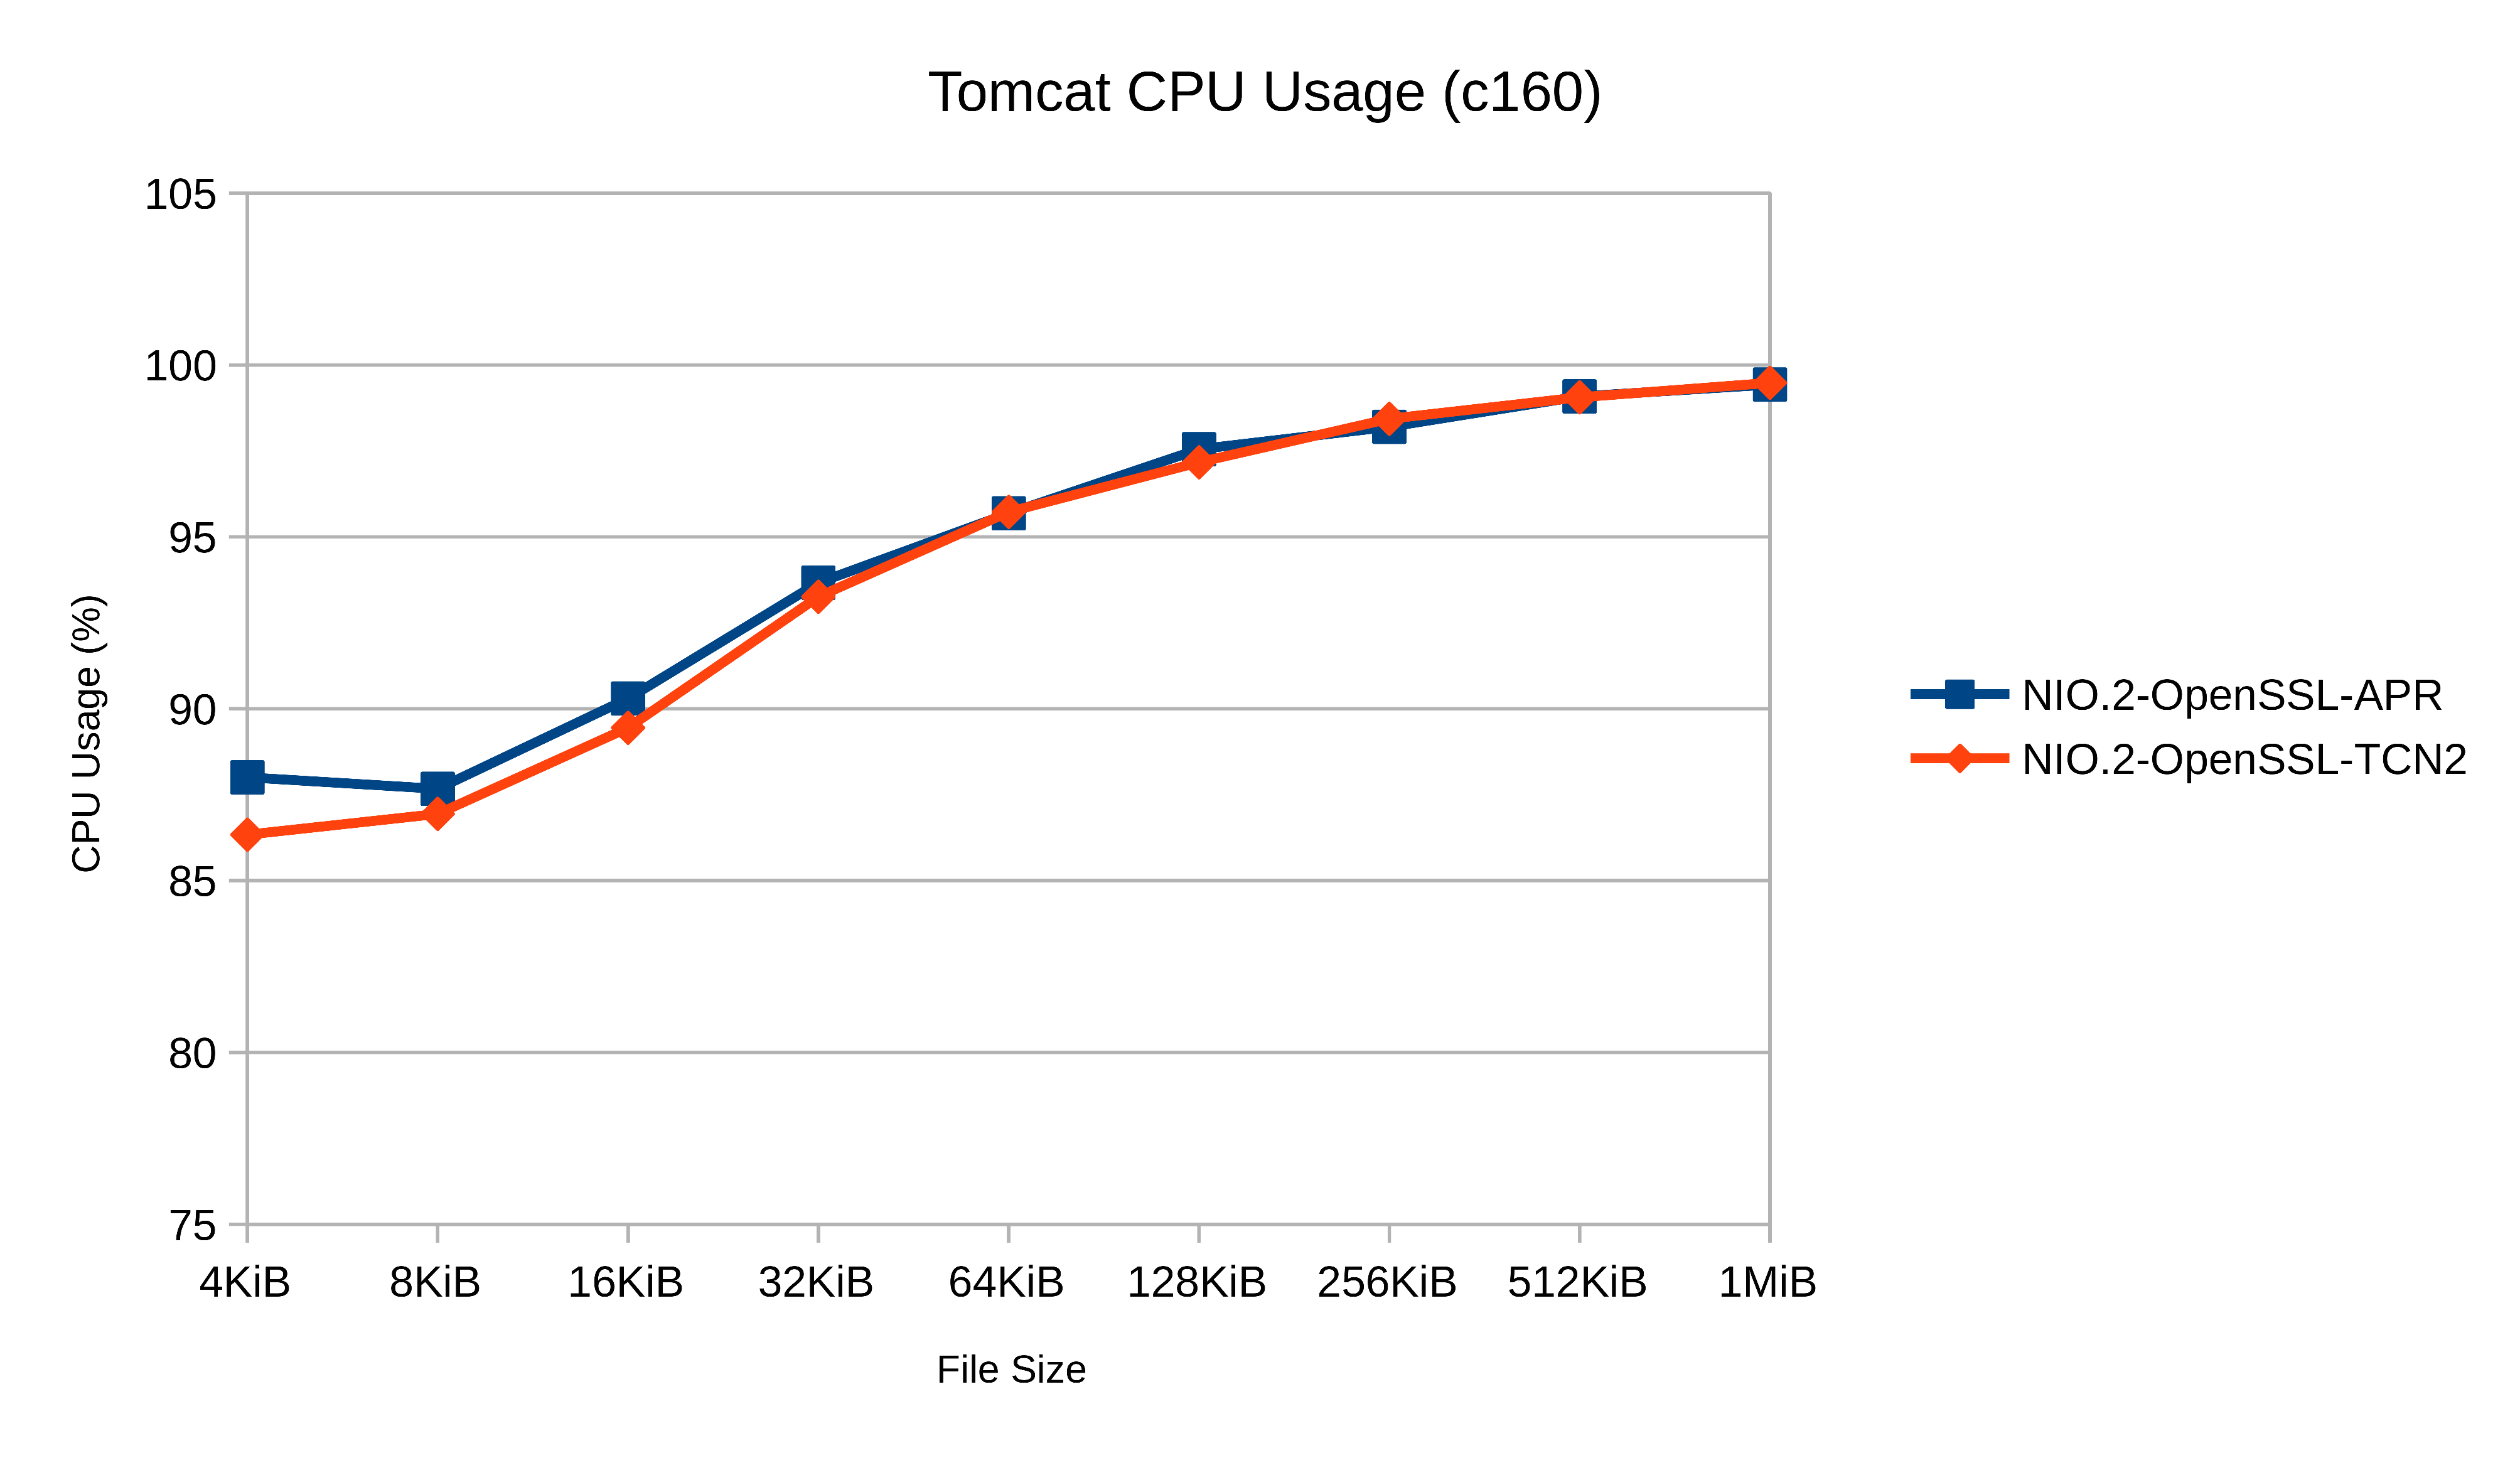
\includegraphics[scale=0.22]{tomcat-cpu.pdf}
	\end{center}
	\caption{\textbf{Diagram showing the difference in CPU usage between Tomcat with \mytitle{} and Tomcat with Tomcat Native.}}
	\label{fig:tomcat-cpu}
\end{figure}

\begin{figure}[!h]
	\begin{center}
		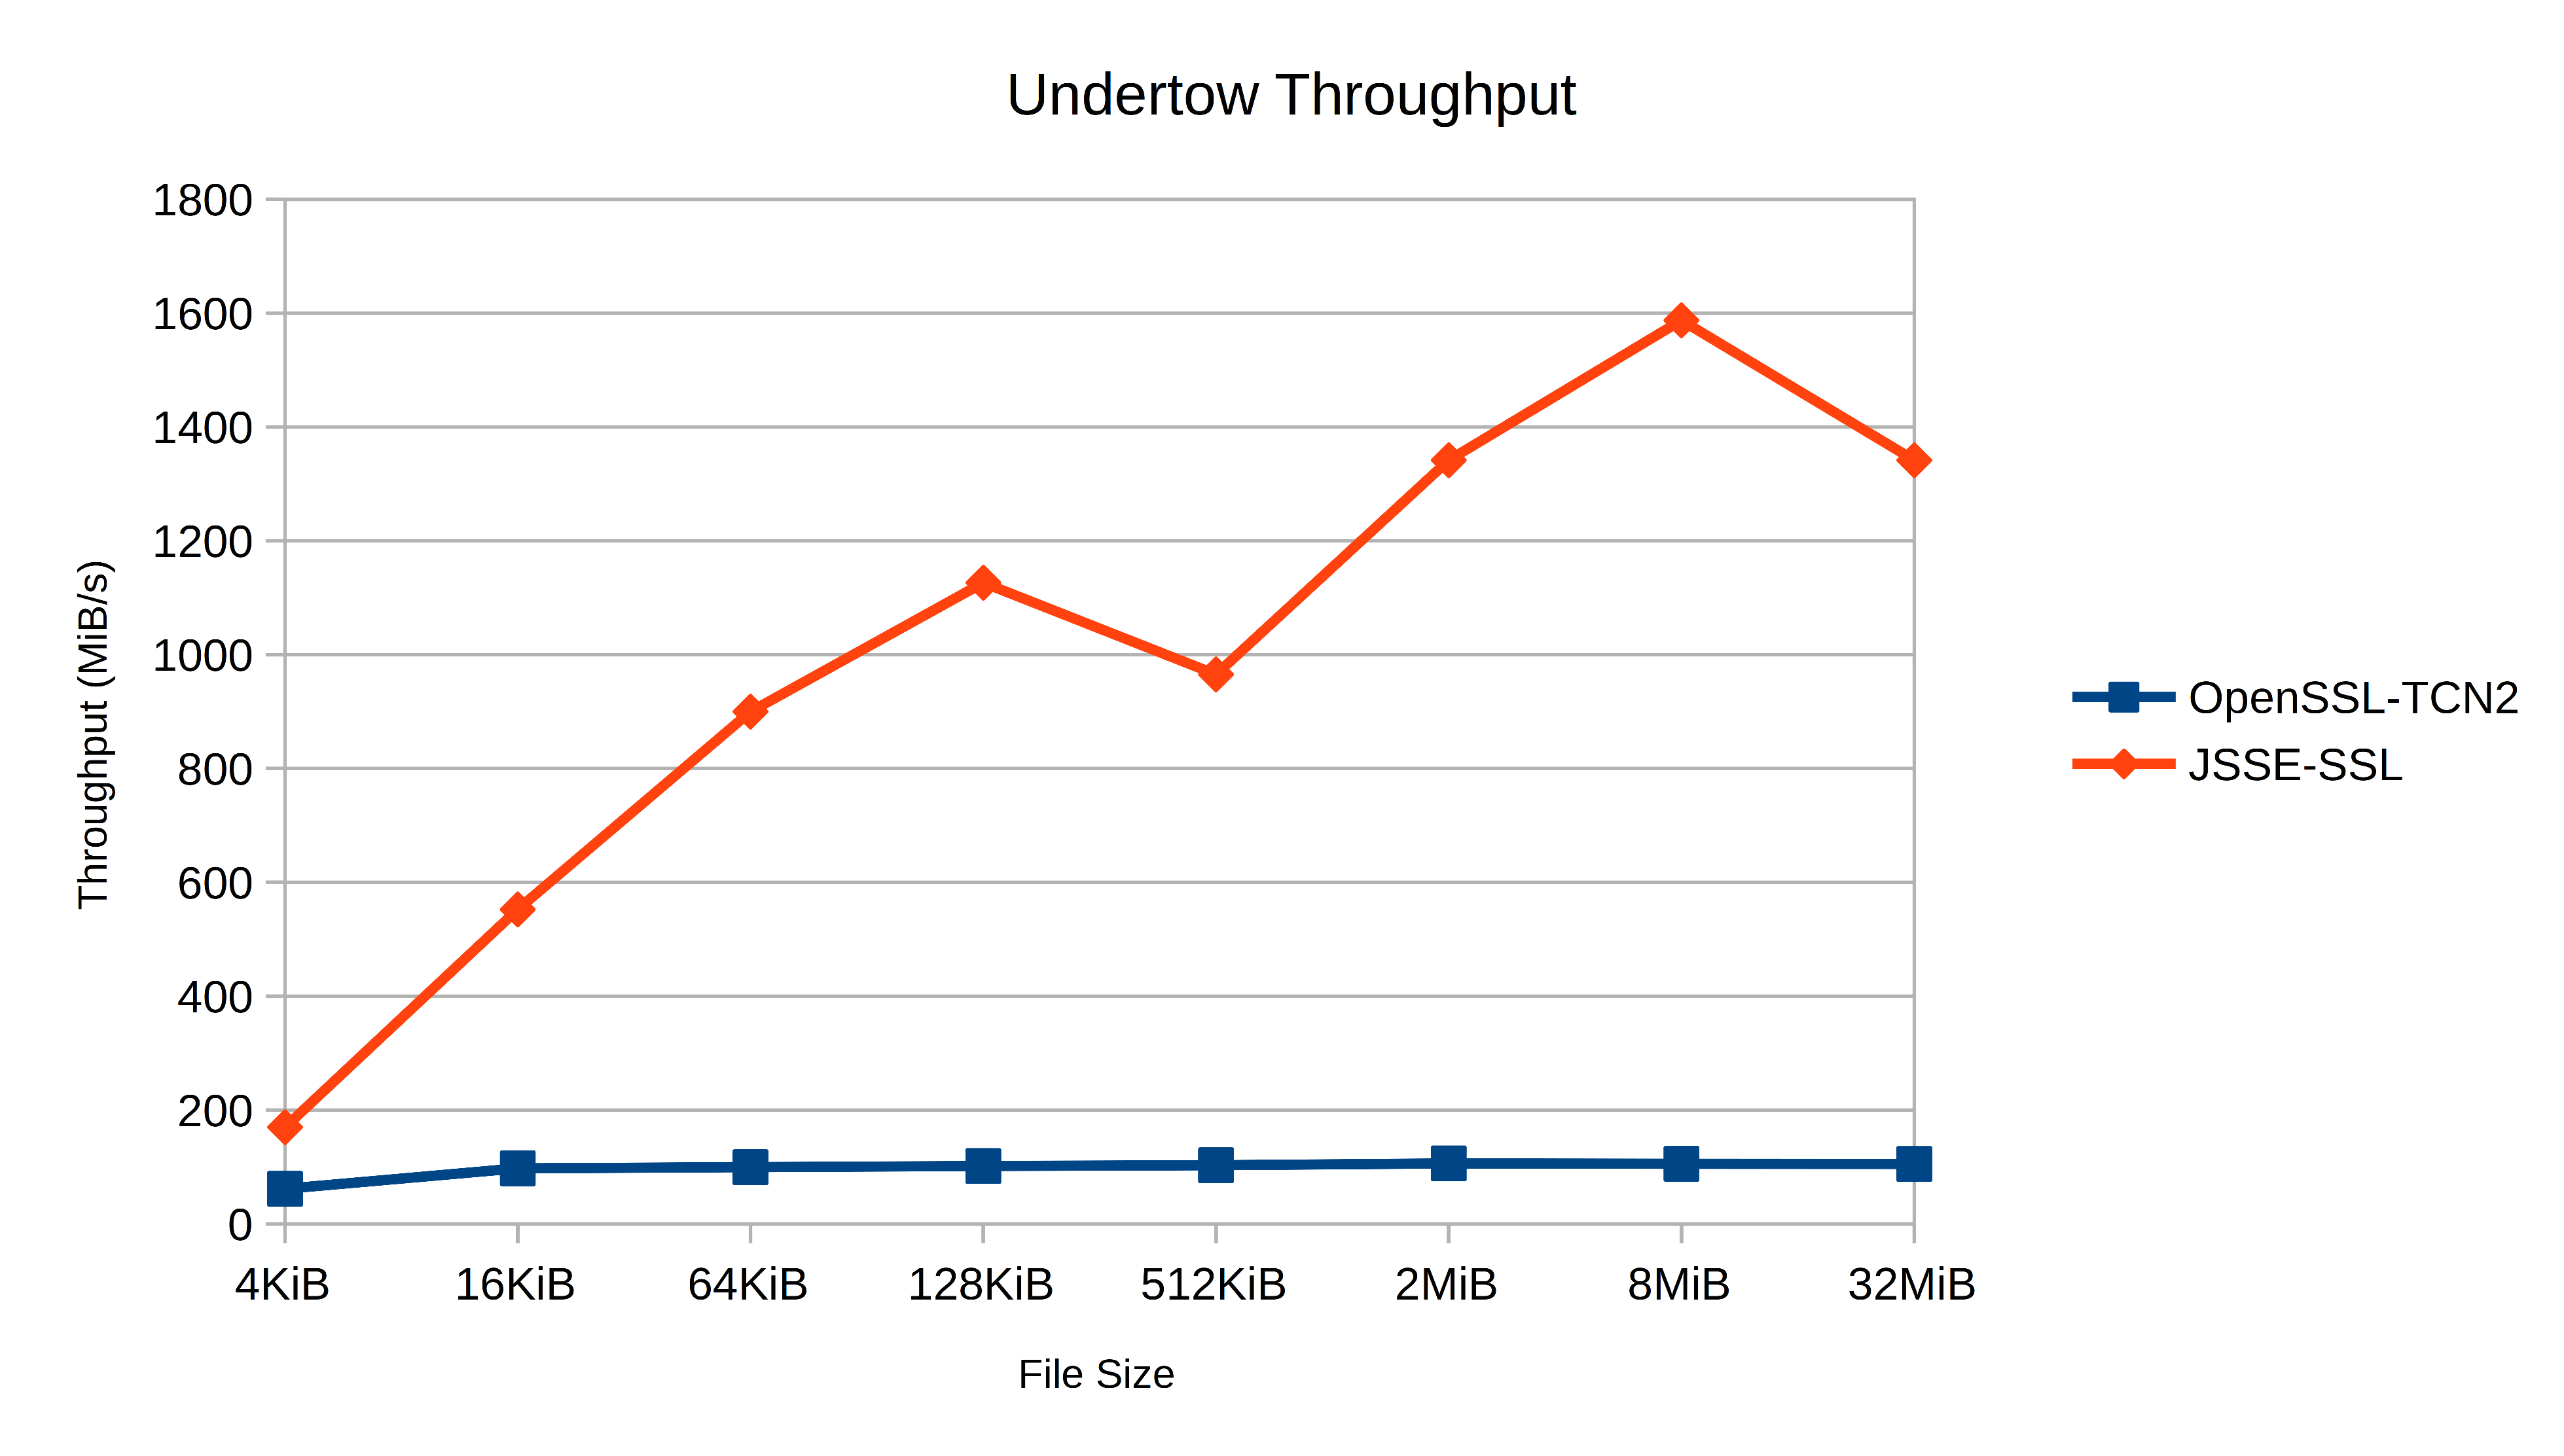
\includegraphics[scale=0.23]{undertow-throughput.pdf}
	\end{center}
	\caption{\textbf{Diagram showing the difference in throughput between Undertow with \mytitle{} and Undertow with the JSSE SSL Engine.}}
	\label{fig:undertow-throughput}
\end{figure}

\FloatBarrier
\section{Issues}
\label{sec:issues}
During this project, we face two issues described in the following subsections.
\subsection{Diverging Philosophies}
When we made \mytitle{} Compatible we wanted to have everything in common in the Java code between Undertow and Tomcat. Unfortunately this was not possible due to diverging opinions between the Tomcat and Undertow maintainers. This concerned the way the OpenSSL engine is provided and instantiated in both project. Undertow maintainers want to use the SPI\footnote{Security Provider Interfaces}, as suggested by JSSE. Tomcat already uses a custom system, which maintainers think is more practical for their usage.

Fortunately, this covered much less code than we imagined although it forced us to rethink some parts of our architecture, in particular how all components would connect with each other.
\subsection{Dynamic Loading}
Some experiments regarding dynamic loading were performed in the \texttt{dynload} branch of our \mytitle{} repository. This would enable \mytitle{} to swap OpenSSL for other TLS/SSL libraries such as LibreSSL or BoringSSL without having to recompile.

 Unfortunately developing a functional prototype with dynamic loading was taking too long, to the detriment of the rest of the project. We therefore made the decision to stop working on this feature.

\section{Future Works}
We completed all the obligatory milestones of the projects. However, some optional tasks were either not started or not finished.

The current code is only a prototype. In the future, tests should be put in place to ensure the code is working as expected in every situations. \mytitle{} should also have a streamlined build process. This should be done when it is eventually merged in Tomcat and Undertow.

\subsection{Better integration}
Some improvements should be made regarding the integration of \mytitle{} in Tomcat and Undertow, in addition to a better build process.

For example, in Undertow we handle ALPN\footnote{Application-Layer Protocol Negotiation} such that HTTP/2 is preferred, even when the underlying server does not support it.

Moreover, we want \mytitle{} to be an optional run-time dependency. However Tomcat currently requires it both at compilation and run-time. Similarly we needed a few classes both in Tomcat and \mytitle{}, so we duplicated them in both projects. We did this to avoid a circular dependency between both projects, but there is a better way.

\subsection{Dynamic Loading}
We unfortunately could not find the time to finish dynamic loading as this proved to be more complicated than we anticipated as stated in section \ref{sec:issues}.

In the future adding Dynamic Loading to \mytitle{} could be a boon for the project.

\subsection{SSL/TLS Integration}
At the moment \mytitle{} does not support the use of sessions. This was not needed to have a working prototype, especially since sessions were not well supported in Tomcat to begin with. However, support of sessions is required for a complete SSL library.

Support for OpenSSL handshake callback should be implemented down the line. Currently we rely on a hack to make it work.
\newpage
\printbibliography

\begin{figure}[!h]
	\begin{center}
		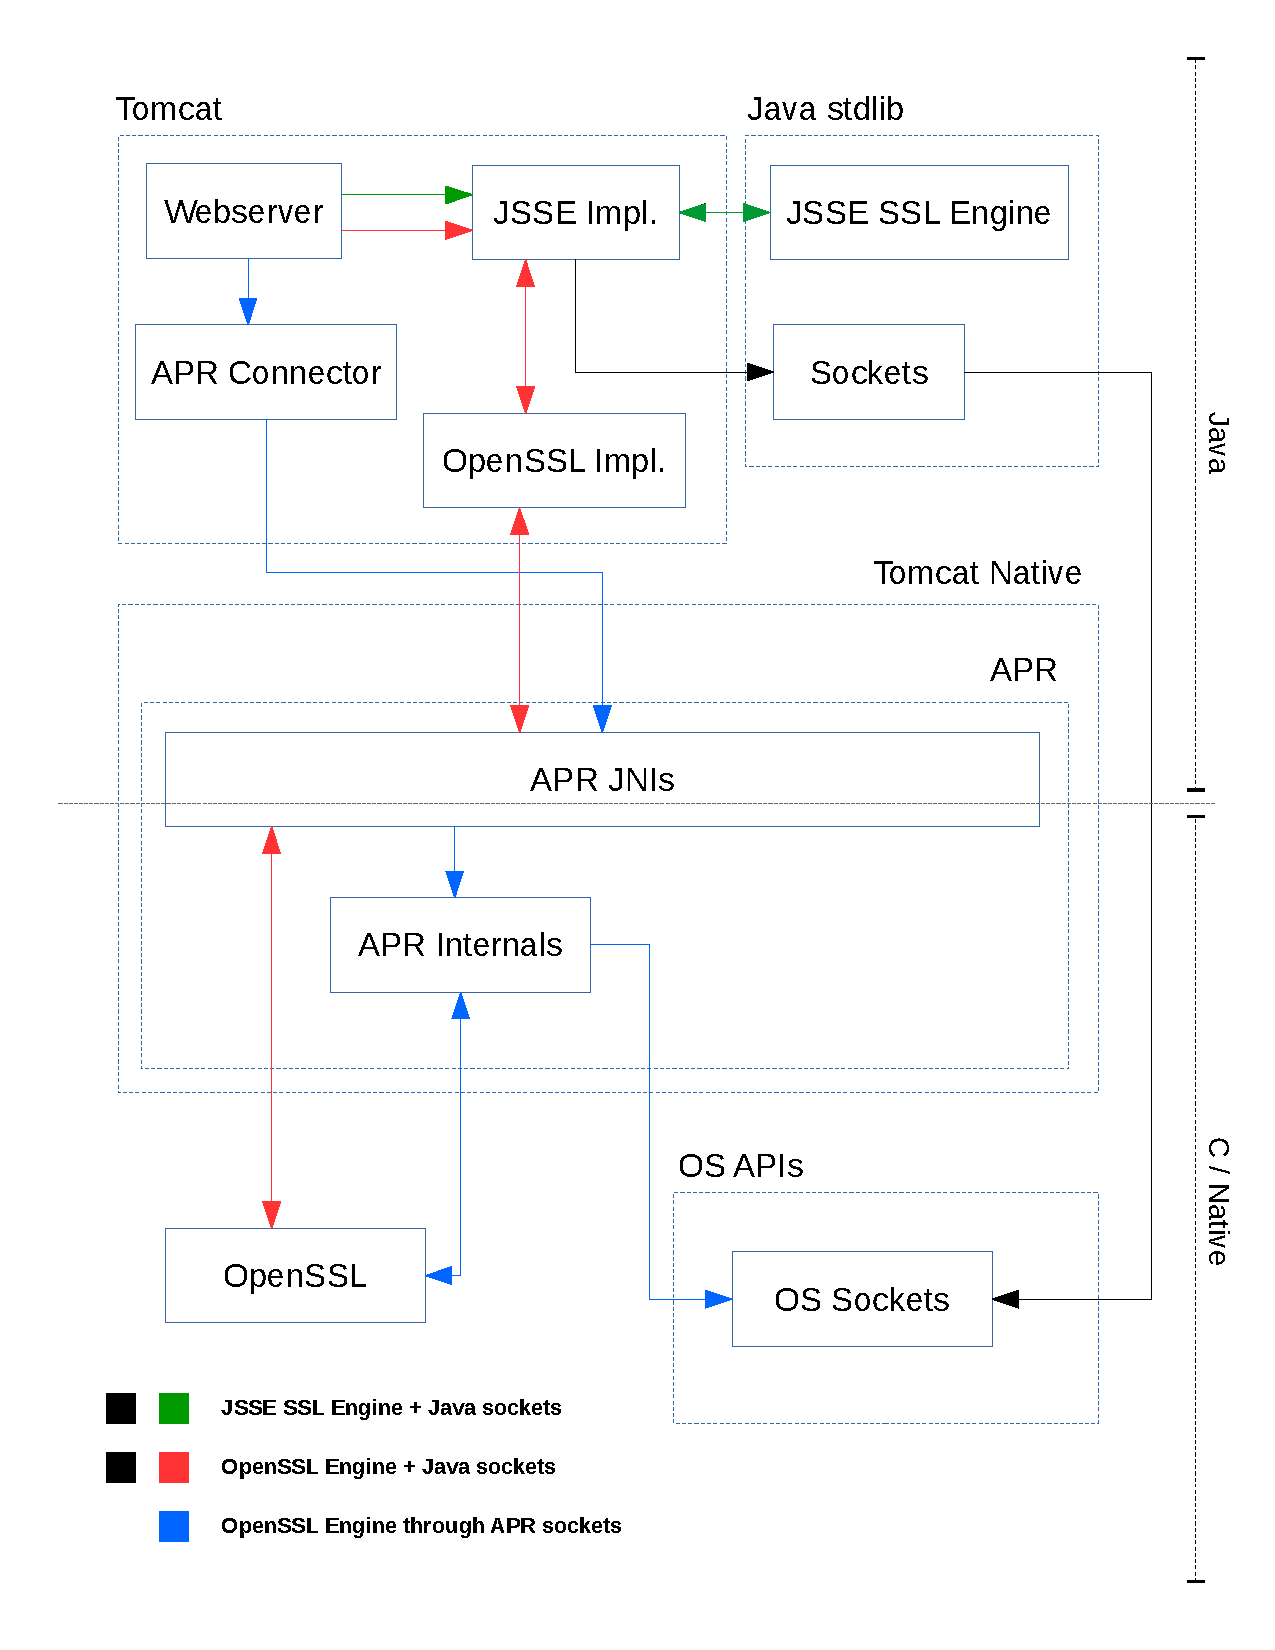
\includegraphics[scale=0.7]{diagram_current_way.pdf}
	\end{center}
	\caption{\textbf{Diagram showing the different ways to use TLS/SSL in Tomcat.}}
	\label{fig:current}
\end{figure}

\begin{figure}[!h]
	\begin{center}
		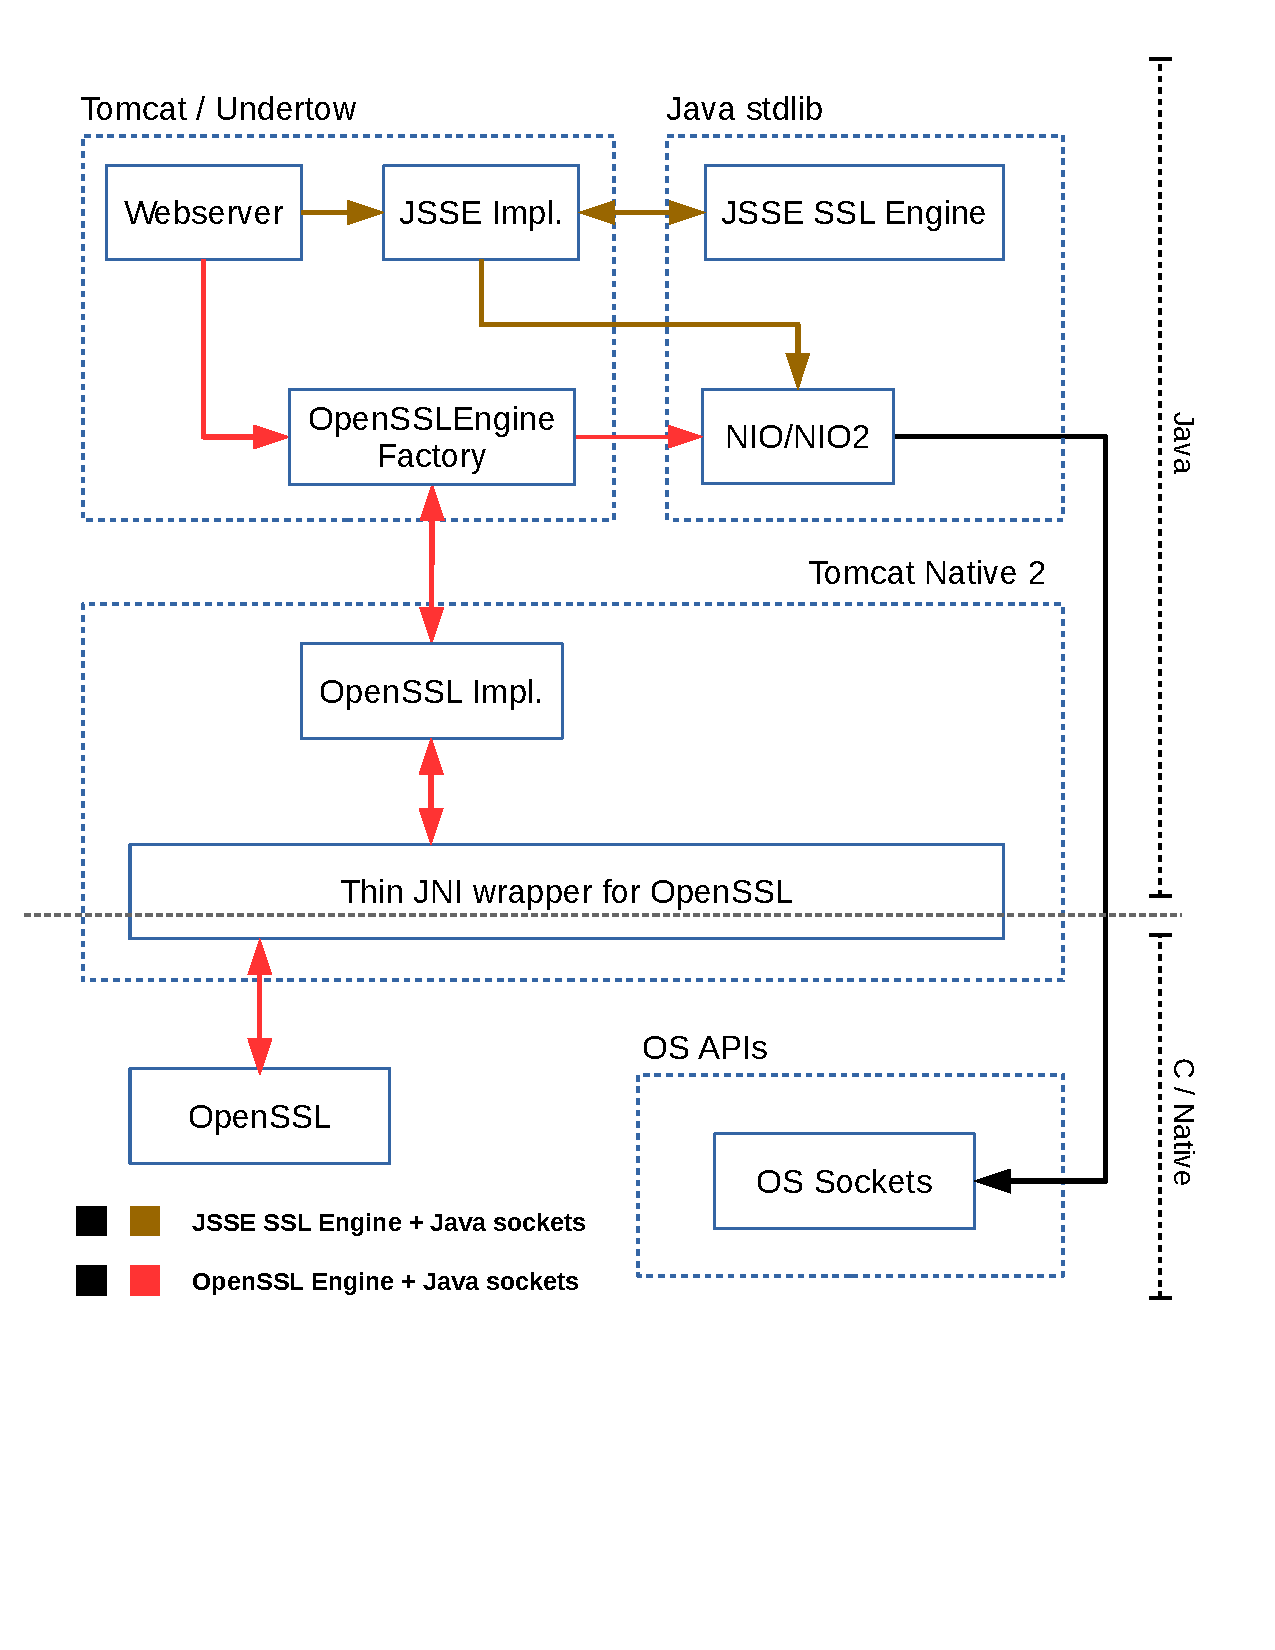
\includegraphics[scale=0.7]{diagram_goal.pdf}
	\end{center}
	\caption{\textbf{Diagram showing the end result of our project.}}
	\label{fig:goal}
\end{figure}

\FloatBarrier

\end{document}